\documentclass{beamer}
\usepackage{tikz}
\usepackage[T2A]{fontenc}
\usepackage[all]{xy}
\usepackage[utf8]{inputenc}
\usepackage[russian]{babel}
\usepackage{hyphenat}
\usepackage[T2A,T1]{fontenc}
\usepackage{amsmath}
\usepackage{graphicx}

\usetheme{Madrid}

\title{Сети и потоки. Алгоритм Диница}

\author{~Кононов Николай}

\institute[СПБГУ]
{
    Математико-Механический факультет СПбГУ
}
\date{2019}

\AtBeginSubsection[]
{
  \begin{frame}<beamer>{План}
    \tableofcontents[currentsection,currentsubsection]
  \end{frame}
}

\begin{document}

\begin{frame}
  \titlepage
\end{frame}

\begin{frame}{План}
  \tableofcontents
\end{frame}


\section{Сети и потоки}

\subsection{Простейшие понятия}

\begin{frame}{Сеть}
  \begin{itemize}
  \item {
    \textbf{Определение: } Пусть есть множество вершин V, в котором выделены две вершины: s (вход или исток) и t (выход или сток). \\Пусть определена функция $c:V \times V \rightarrow \mathbb{R}$, удовлетворяющая соотношениям $$\forall x, y \in V \quad c(x, y) \geq 0, \quad c(x, s) = 0, \quad c(t, y) = 0 $$
    функция $c$ - \textbf{пропускная способность}.
    \pause
  }
  \item {
    $A = \{(x, y) : c(x, y) > 0\}$ - множество стрелок\\  Тогда $ G = ((V, A), s, t, c) $ - \textbf{сеть}
  }
  \end{itemize}
\end{frame}

% You can reveal the parts of a slide one at a time
% with the \pause command:
\begin{frame}{Поток в сети}
  \begin{itemize}
  \item {
    \textbf{Определение: } Пусть $G - $ сеть, а функция $f:V \times V \rightarrow \mathbb{R}$ удовлетворяет трем условиям:\\
        1) $\forall x, y \in V \quad f(x, y) \leq c(x, y)$\\
        2) $\forall x, y \in V \quad f(x, y) = -f(y, x)$\\
        3) $\forall v \in V\textbackslash \{s, t\}$ выполняется условие: $ \sum\limits_{x \in V} f(v, x) = 0$ - закон сохранения потока
    \\ $f$ - \textbf{поток в сети $G$}
    \pause
  }
  \item {
    $ |f| = \sum\limits_{v \in V} f(s, v)$ - величина потока\\
        Поток с максимальной величиной - \textbf{максимальный}
  }
  \end{itemize}
\end{frame}

\begin{frame}{Разрез сети}
  \begin{itemize}
    \item {
        \textbf{Определение: } пусть $G$ - сеть, а множество ее вершин $V$ разбито на два дизъюнктых множества $S \ni s$ и $T \ni t$. Тогда $(S,T)$ - \textbf{разрез сети G}
        \pause
    }
    \item {
        Величина $c(S, T) =  \sum\limits_{x \in S, y \in T}c(x, y)$ называется \textbf{пропускной способностью разреза}. \\ Любой разрез сети G с минимальной пропускной способностью называется \textbf{минимальным}.
        \pause
    }
    \item {
        Для любого потока f величина $f(S, T) =  \sum\limits_{x \in S, y \in T} f(x, y)$ называется \textbf{потоком через разрез}.
        \pause
    }
    \end{itemize}
    \begin{block}{Лемма}
        \textbf{Лемма: } Для любого потока $f$, и разреза $(S, T)$ сети $G$ выполняется $|f| = f(S, T)$
    \end{block}
\end{frame}

\subsection{Остаточная сеть, блокирующий поток}

\begin{frame}{Остаточная сеть}
    \begin{itemize}
    \item {
        \textbf{Остаточной пропускной способностью} $c_{f}$ по отношению к сети $G = \{(V, E), s, t, c\}$ и потоку $f$ в ней называется пропускная способность
        \begin{equation*}
        c_{f}(x, y) = 
         \begin{cases}
           0 &\text{if y = s or x = t}\\
           c(x, y) - f(x, y) &\text{otherwise}
         \end{cases}
        \end{equation*}
        \\
        \pause
    }
    \item {
        \textbf{Остаточной сетью} для сети $G$ и потока $f$ называется сеть $G_{f} = \{(V, E_{f}), s, t, c_{f}\}$, где $E_{f} = \{ (u, v) \in V \times V | c_{f}(u, v) > 0\}$
    }
    \item {
        Остаточное ребро можно интуитивно понимать как меру того, насколько можно еще увеличить поток вдоль этого ребра
        \pause
    }
    \begin{exampleblock}{Определение}
    Простой st-путь в $G_{f}$ называется \textbf{дополняющим путем}
    \end{exampleblock}

    \end{itemize}
\end{frame}

\begin{frame}{Блокирующий поток}
    \small {
    \begin{exampleblock}{Определение}
        \textbf{Блокирующим потоком $f$} в сети $G = ((V, E), s, t, c)$ называется такой поток, что $\forall st$-путь содержит насыщенное этим потоком ребро. То есть в данной сети не найдется такого пути из истока в сток, вдоль которого можно безпрепятственно увеличить поток 
    \end{exampleblock}
    \textbf{Замечание: } блокирующий поток не всегда максимальный, более того, он может быть сколь угодно малым, относительно максимального \\
    \pause
    \textbf{Пример:} пропускная способность ребер 1, 
        'единичный' поток идет по красным ребрам
    }
    \begin{figure}[h!]
        \advance\leftskip-3cm
        \advance\rightskip-3cm

        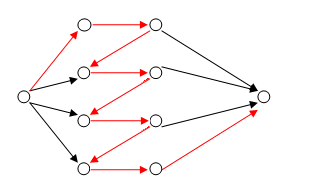
\includegraphics[scale=0.7]{blocking_flow.png}
        \label{fig: blocking_flow}
    \end{figure}
\end{frame}

\subsection{Теорема Форда-Фалкерсона}
\begin{frame}{Теорема Форда-Фалкерсона}
    \begin{theorem}
        \textbf{Ford-Fulkerson:} В сети $G$ с пропускной способностью $c$ задан поток $f$, тогда \textit{следующие три утверждения равносильны:\\
        1) Поток f максимален\\
        2) $\exists (S, T)$ : $|f| = c(S, T)$\\
        3) В остаточной сети $G_f$ нет дополняющего пути
        }
    \end{theorem}
\end{frame}

\subsection{Слоистая сеть}

\begin{frame}{Слоистая сеть}
    \textbf{Слоистая сеть(layered network, вспомогательная сеть)} строится след образом:
    \begin{itemize}
        \item {
            Для каждой вершины $v$ данной сети $G$ определим длину кратчайшего $s \rightsquigearrow v$-пути из истока и обозначим ее \texttt{d[v]} (можно сделать обходом в ширину)
        }
        \item {
            В слоистую сеть включаем только стрелки $(u, v)$ такие, что \texttt{d[u] = d[v] + 1}
        }
        \item {
            То есть исключим из $G$ стрелки лежащие внутри одного уровня или идущие назад
        }
        \item {
            Получившаяся сеть ациклична и любой $s \rightsquigarrow t$ путь в слоистой сети является кратчайшим путем в исходной сети из свойств \textbf{BFS}
        }
        \item {
         $ G = \{\{1, 2\}, \{3\}, \{4\}, \{2, 5\}, \{3, 5\}, \{1, 6\}\}; \quad s = 0, t = 6$
         \\тогда \textbf{слоистая сеть $G_{s}$} = $\{\{1, 2\}, \{3\}, \{4\}, \{5\}, \{5\}, \{6\}\}$
        }
    \end{itemize}
\end{frame}

\begin{frame}{Пример слоистой сети}
    \begin{figure}[h!]
        \centering
        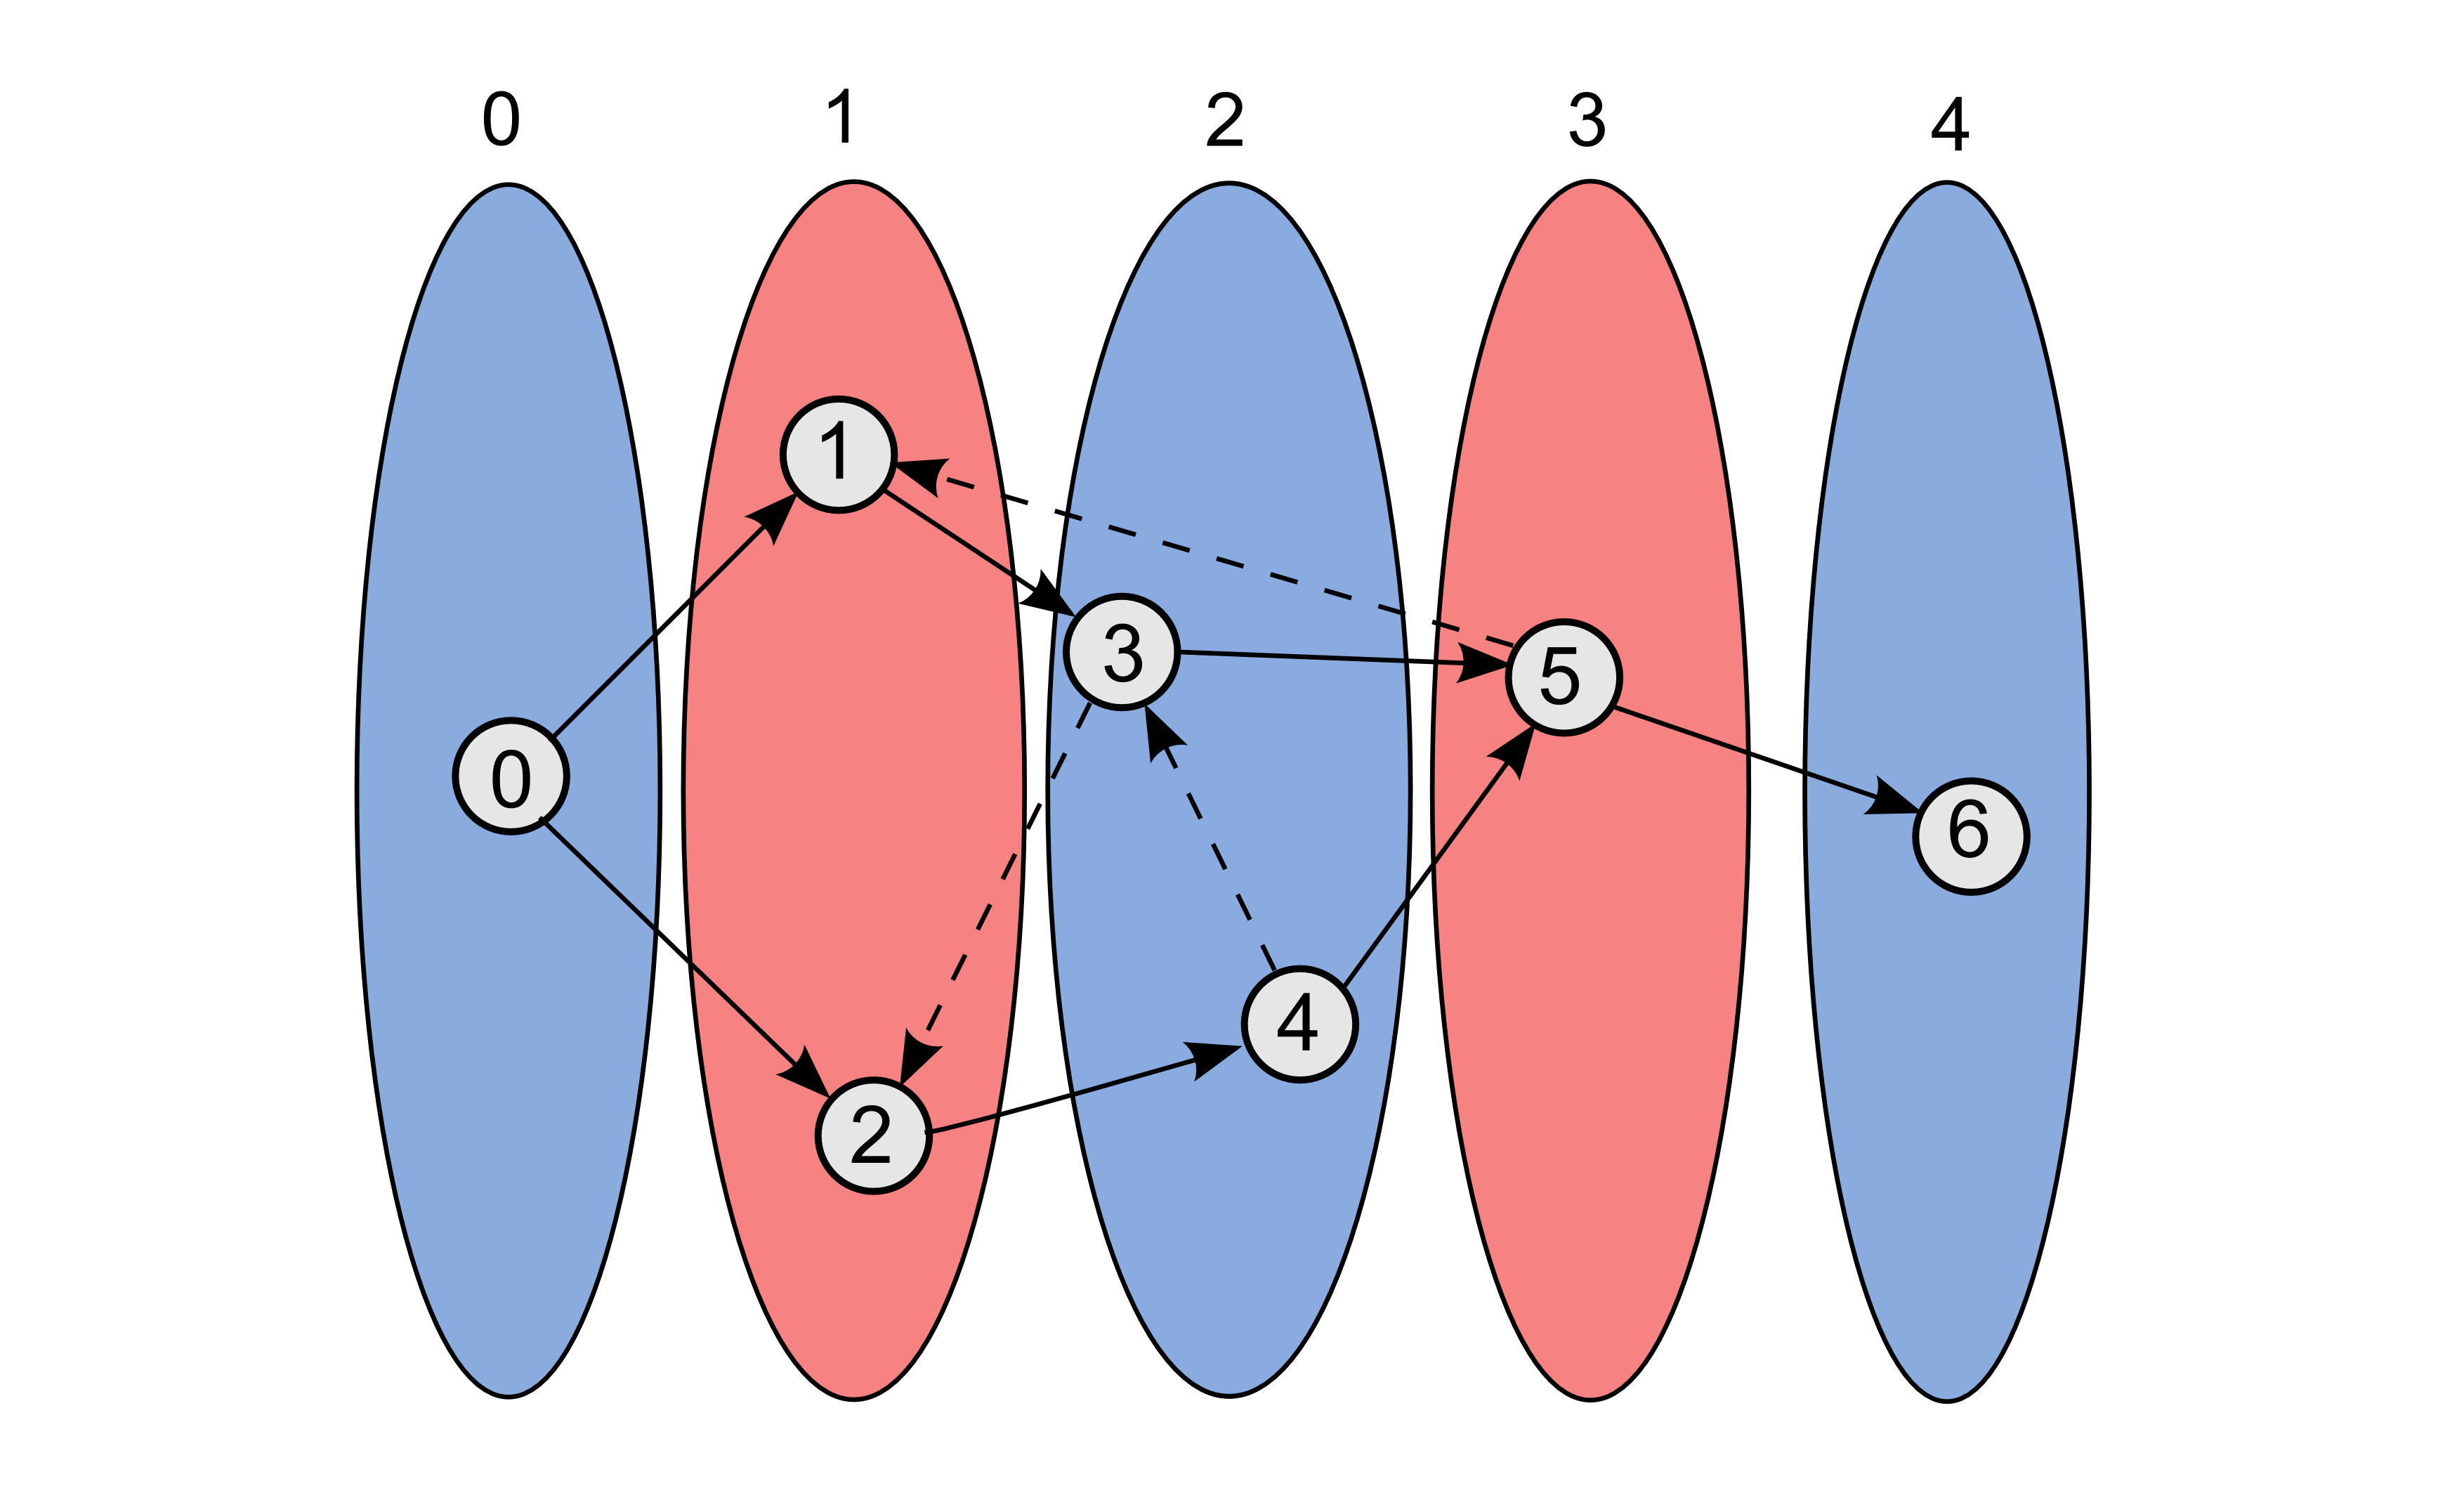
\includegraphics[scale=0.4]{network.png}
        \label{fig: blocking_flow}
    \end{figure}
\end{frame}

\section{Алгоритм Диница}

\subsection{Основные идеи}

\begin{frame}{Алгоритм Диница. Основные идеи}
    \begin{block}{Постановка задачи}
    Пусть дана сеть $G = ((V, E), s, t, c)$. Как найти поток $f$ из $s$ в $t$ максимальной величины?
    \end{block}
    \begin{itemize}
        \item {
        Алгоритм является улучшенной версией \textbf{Алгоритма Эдмонса-Карпа}
        \pause
        }
        \item {
        Изначально пусть $f(e) = 0 \quad \forall e \in E$
        \pause
        }
        \item {
        Алгоритм состоит из нескольких \textbf{фаз}.
        \pause
        }
        \item {
        На каждой фазе строится остаточная сеть \textbf{$G_f$}, затем по отношению к $G_f$ строится слоистая сеть $G_{L}$(\textbf{BFS}). 
        
        Если \texttt{d[t] = $\infty$} останавливаемся и выводим $f$
        \pause
        }
        \item {
        В построенной слоистой сети находим блокирующий поток $f`$ (любой)
        \pause
        }
        \item {
        Дополняем поток $f$ потоком $f`$ и переходим к следующей фазе
        }
    \end{itemize}
\end{frame}

\subsection{Пример}
\begin{frame}{Пример}
    \begin{itemize}
    \item {
        f = 0
    }
    \item {
            $(G, f) \rightarrow G_{f} \rightarrow G_{L} \rightarrow f' \rightarrow f = f + f`$
        }
    \end{itemize}

    \begin{figure}[h!]
        \centering
        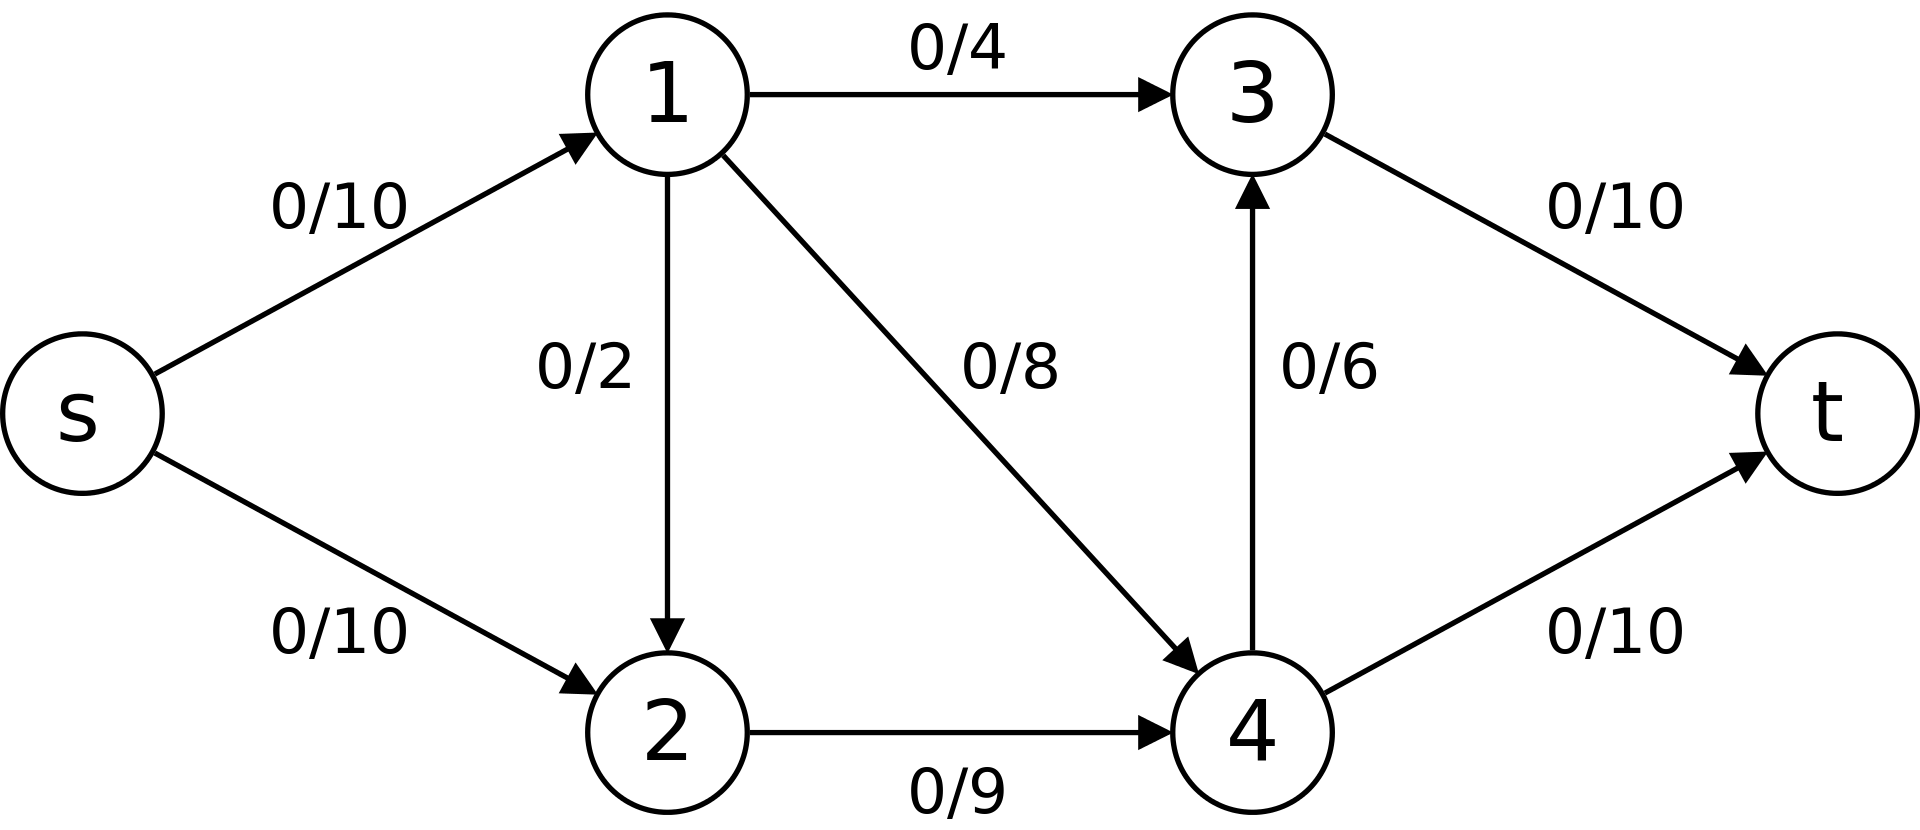
\includegraphics[scale=0.15]{Dinic_algorithm_G1.png}
        \label{fig: example}
    \end{figure}
\end{frame}

\subsection{Корректность}
\begin{frame}{Корректность алгоритма}
    \begin{theorem}
        Если алгоритм завершается, полученный поток является потоком максимальной длины.
    \end{theorem}
    \pause
    \begin{proof}
        Предположим, что в какой-то момент в слоистой сети $G_{L}$ построенной для остаточной сети $G_f$ не удалось найти блокирующий поток.\\
        \pause
        Это означает, что $\texttt{d[t] = } \infty$, то есть сток $t$ не достижим из истока $s$ в слоистой сети .\\
        \pause
        Но слоистая сеть содержит в себе все кратчайшие пути в сети $G_{f}$ из истока $s$.\\
        \pause
        Таким образом в остаточной сети нет 
        $s \rightsquigarrow t$ пути\\
        \pause
        Применяя теорему Форда-Фалкерсона получаем, что текущий поток в самом деле максимален.
    \end{proof}
\end{frame}

\subsection{Асимптотика и оценка числа фаз}

\begin{frame}{Оценка числа фаз}
\begin{lemma}
        Кратчайшее расстояние между истоком и стоком устрого увеличивается с выполнением каждой итерации:
        \texttt{$d_{i}[t] > d_{i-1}[t] $}
    \end{lemma}
    
    \begin{proof}
        От противного. Пусть длина кратчайшего $s \rightsquigarrow t$ пути не изменилась после $i$-ой итерации.
        Слоистая сеть $G_{L}$ строится по остаточной $G_{f}$ 
        
    \end{proof}
\end{frame}

\begin{frame}{Оценка числа фаз}
    \begin{lemma}
        Кратчайшее расстояние от истока до каждой вершины не уменьшается с выполнением каждой итерации:
        \forall v \in V \quad \texttt{$d_{i}[v] \geq d_{i-1}[v] $}
    \end{lemma}
    
    \begin{proof}
        Зафиксируем произвольную вершину $v$ и итерацию $i$ и рассмотрим кратчайший $s \rightsquigarrow v$ путь P в сети $G^{i}_{f}$. Ясно, что $|P| = d_{i}[v]$\\
        \pause
        Заметим, что в остаточную сеть $G^{i}_{f}$
    \end{proof}
\end{frame}

\begin{frame}{Оценка числа фаз}
    \begin{itemize}
    \item {
        Так как длина кратчайшего $s \rightsquigarrow t$ пути не может превосходить $n - 1 \Rightarrow$ алгоритм Диница совершает не больше $n - 1$ фаз (итераций цикла).
        \pause
    }
    \item {
        Таким образом, в зависимости от того, каким алгоритмом нахождения блокирующего потока мы пользовались алгоритм Диница может выполнятся за $O(|V| \cdot |E|^{2})$ или за $O(|V|^{2} \cdot |E|)$\\
        \pause
    }
    \item {
        Возможно достичь асимптотики $O(|V| \cdot |E| \cdot log(|V|)$, используя \textbf{динамические деревья Слетора и Тарьяна}
    }


    \end{itemize}
\end{frame}

\subsection{Поиск блокирующего потока}
\begin{frame}{Поиск блокирующего потока}{$O(|E|^{2})$}
    \begin{itemize}
        \item {
            Так как слоистая сеть $G_{L}$, в которой ищется блокирующий поток ациклическая - будем искать блокирующий поток в ациклической сети.
        }
        \item Искать $s \rightsquigarrow t$ пути по одному, пока такие пути находятся
    \end{itemize}

\end {frame}

\subsection{Реализация}
\begin{frame}{Реализация}
\end{frame}

\begin{frame}[allowframebreaks]
  \frametitle<presentation>{Литература}

  \begin{thebibliography}{10}

  \beamertemplatebookbibitems

  \bibitem{Кормен2007}
    Т.~Кормен.
    \newblock {\em Алгоритмы. Построение и анализ}.
    \newblock Глава 27, "Максимальный поток".


  \beamertemplatearticlebibitems

  \bibitem{}
      ~neerc.ifmo.ru
      \newblock "Схема алгоритма Диница"
  \end{thebibliography}
\end{frame}

\end{document}
